\section{Appendix}
In this section, we analyze the trace plots for the different models implemented. The analysis is consistent across all models due to the similarity of the trace plots. Notably, none of the trace plots display any distinct patterns. Furthermore, they appear to thoroughly explore the entire parameter space, as indicated by frequent transitions into various regions. The following plots were generated using a single chain; however, we have confirmed that the behavior remains consistent when using multiple chains.
\begin{figure}[H]
    \centering
    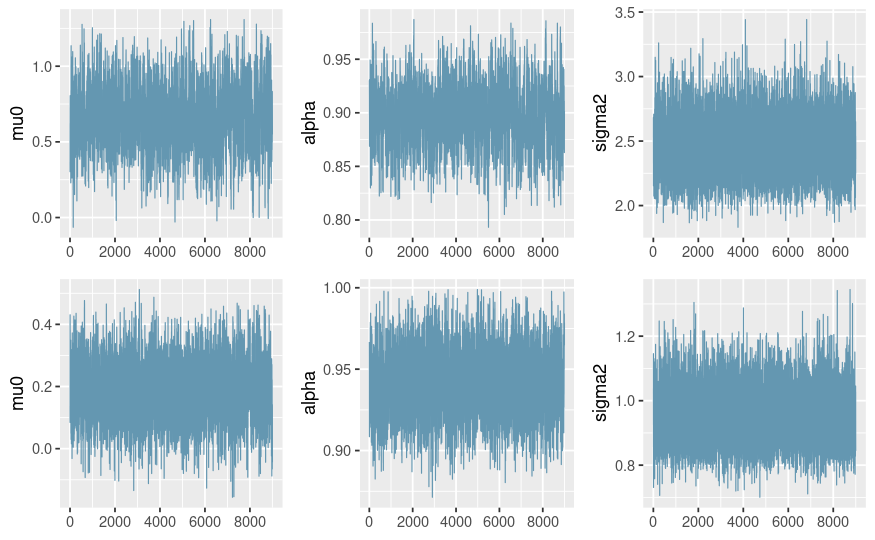
\includegraphics[width=0.9\textwidth]{images/2-AR/traceplots.png}
    \caption{Trace plots for the AR(1) models. The top line corresponds to the model used for GDP, while the bottom line corresponds to the model used for CPIAUCSL.}
\end{figure}
\begin{figure}[H]
    \centering
    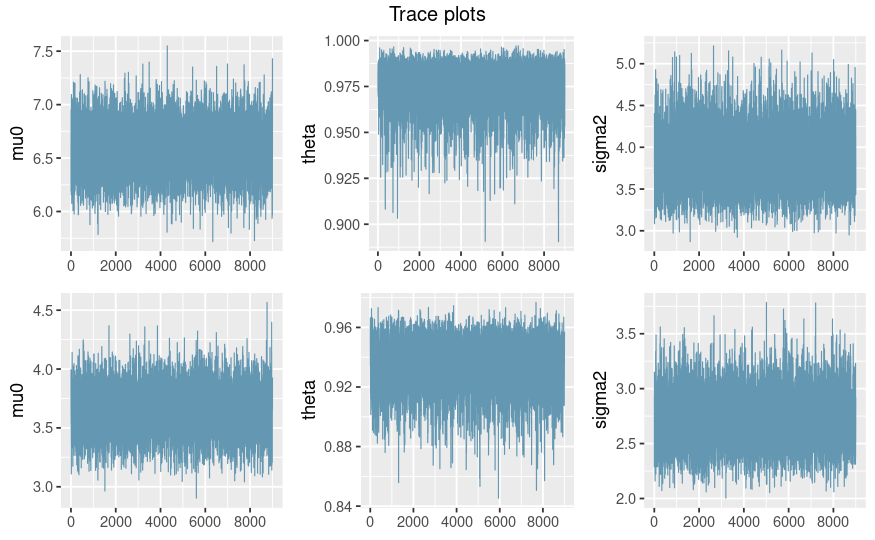
\includegraphics[width=0.9\textwidth]{images/3-MA/traceplots.png}
    \caption{Trace plots for the MA(1) models. The top line corresponds to the model used for GDP, while the bottom line corresponds to the model used for CPIAUCSL.}
\end{figure}
\begin{figure}[H]
    \centering
    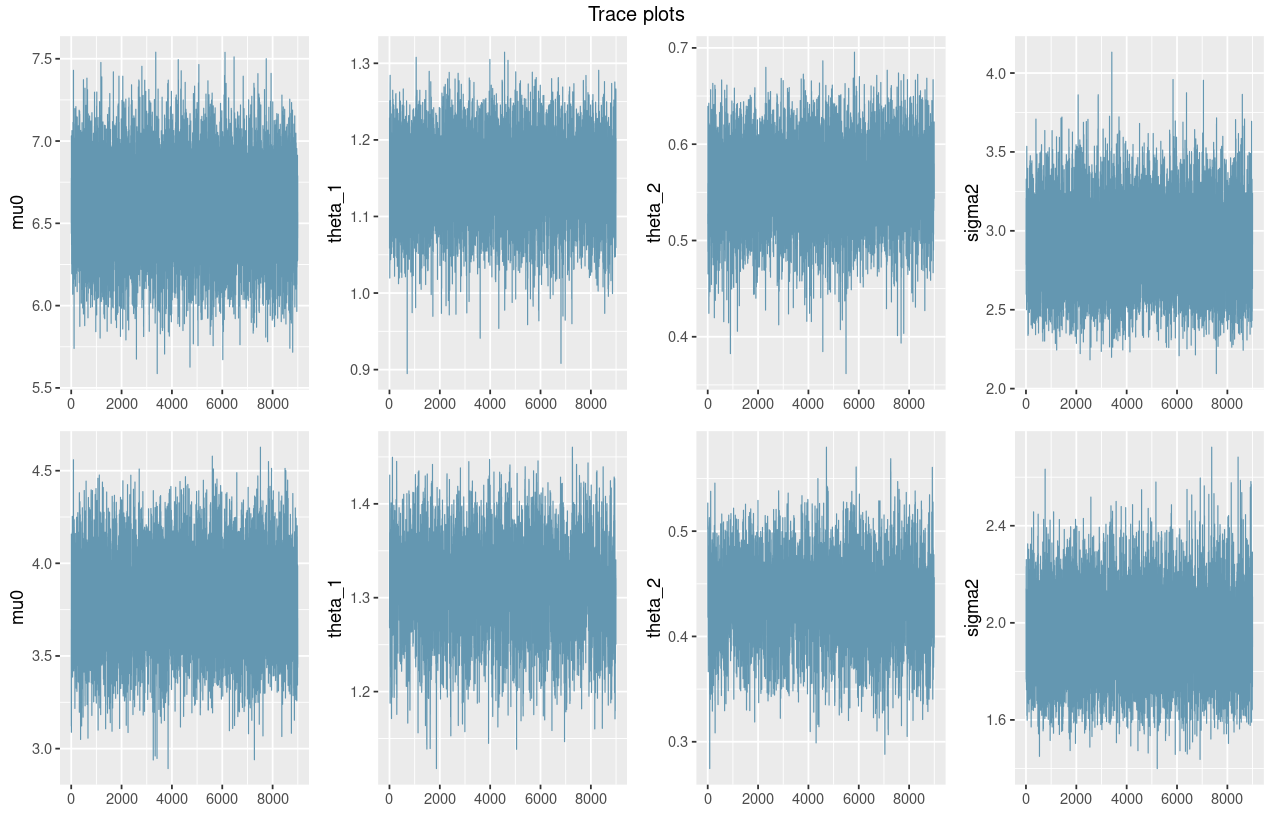
\includegraphics[width=0.9\textwidth]{images/3-MA/traceplots2.png}
    \caption{Trace plots for the MA(2) models. The top line corresponds to the model used for GDP, while the bottom line corresponds to the model used for CPIAUCSL.}
\end{figure}
\begin{figure}[H]
    \centering
    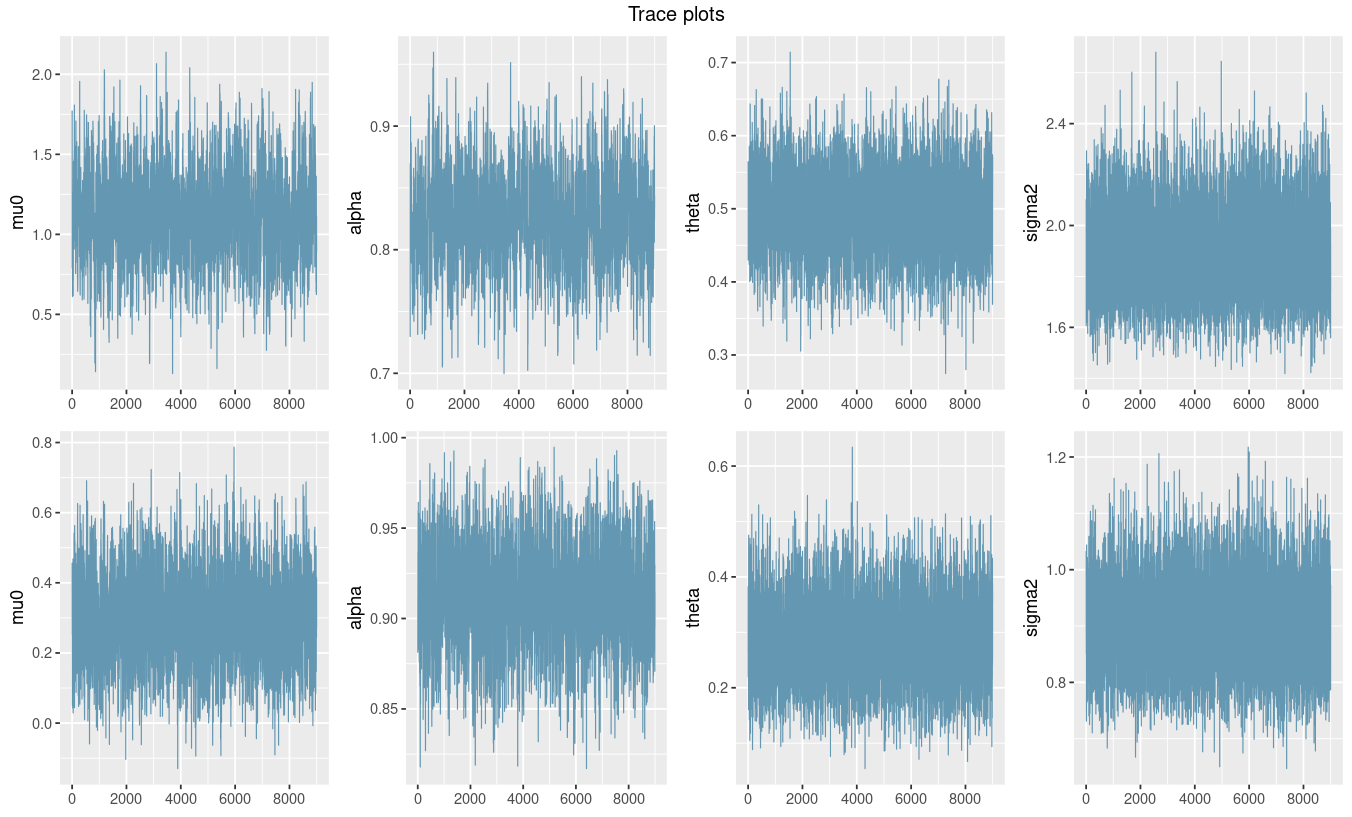
\includegraphics[width=0.9\textwidth]{images/4-ARMA/traceplots.png}
    \caption{Trace plots for the ARMA(1,1) models. The top line corresponds to the model used for GDP, while the bottom line corresponds to the model used for CPIAUCSL.}
\end{figure}
\begin{figure}[H]
    \centering
    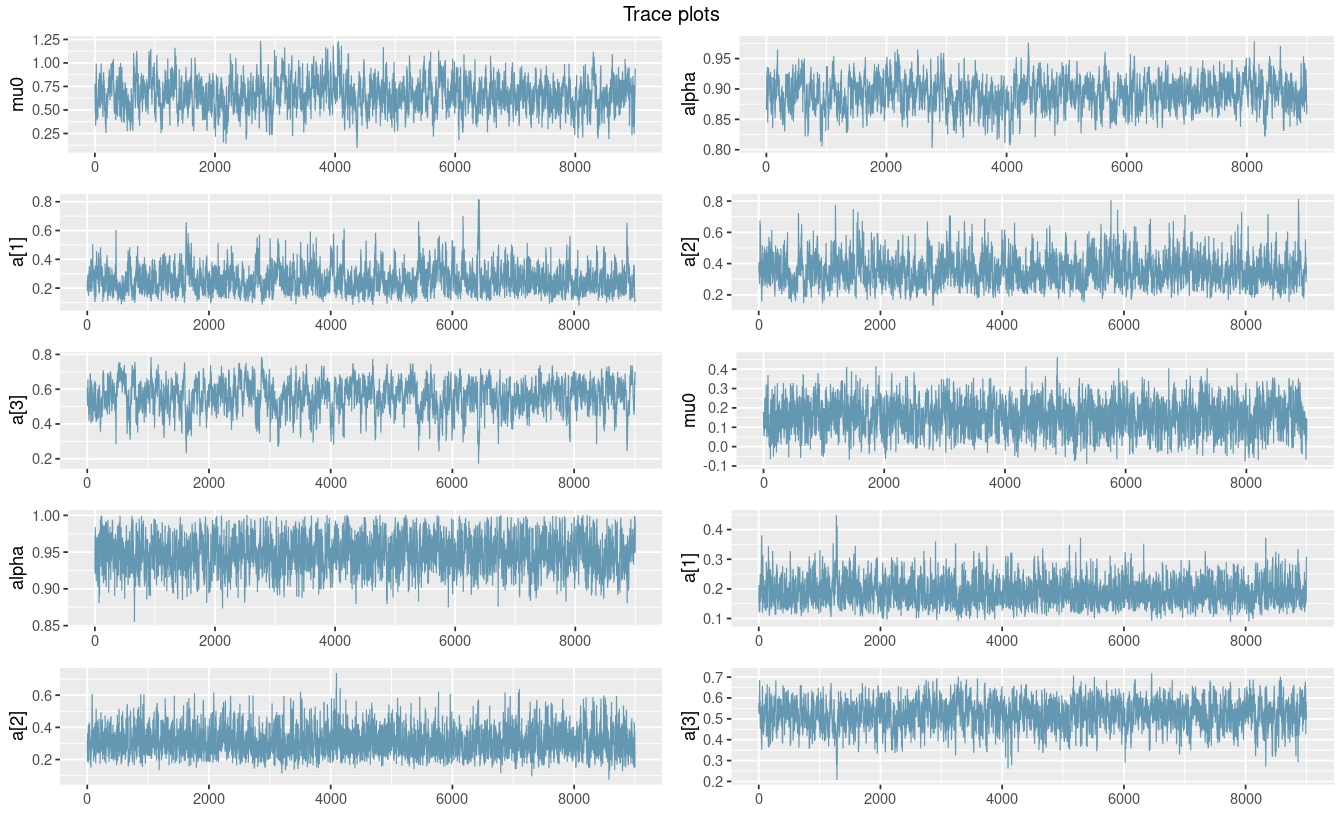
\includegraphics[width=0.9\textwidth]{images/5-GARCH/traceplots.png}
    \caption{Trace plots for the AR(1) + GARCH(1,1) models. The top line corresponds to the model used for GDP, while the bottom line corresponds to the model used for CPIAUCSL.}
\end{figure}
\begin{figure}[H]
    \centering
    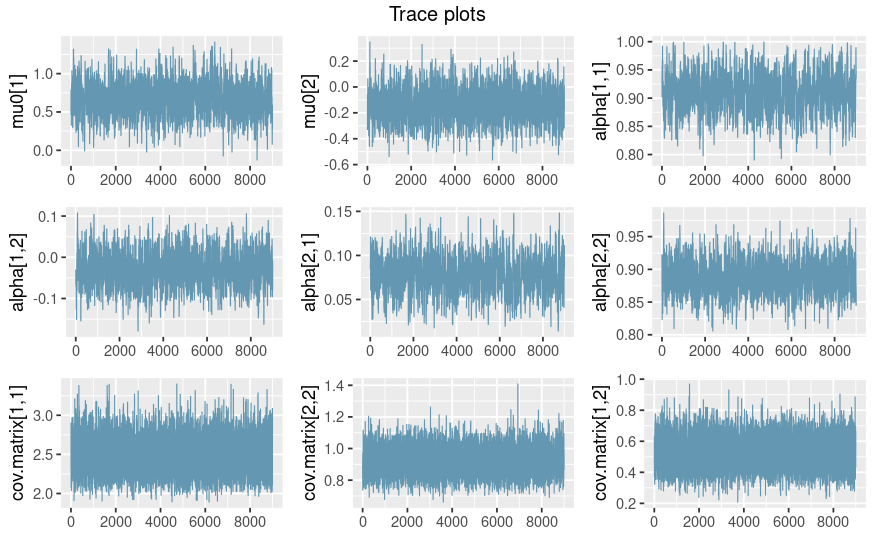
\includegraphics[width=0.9\textwidth]{images/6-VAR/traceplots.png}
    \caption{Trace plots for the VAR(1) model.}
\end{figure}